%%% LaTeX Template: Designer's CV
%%%
%%% Source: http://www.howtotex.com/
%%% Feel free to distribute this template, but please keep the referal to HowToTeX.com.
%%% Date: March 2012


%%%%%%%%%%%%%%%%%%%%%%%%%%%%%%%%%%%%%
% Document properties and packages
%%%%%%%%%%%%%%%%%%%%%%%%%%%%%%%%%%%%%
\documentclass[letterpaper,12pt,final]{memoir}

% misc
\renewcommand{\familydefault}{bch}	% font
\pagestyle{empty}					% no pagenumbering
\setlength{\parindent}{0pt}			% no paragraph indentation


% required packages (add your own)
\usepackage{flowfram}										% column layout
\usepackage[top=1cm,left=0.2cm,right=1cm,bottom=0.8cm]{geometry}% margins
\usepackage{graphicx}
\usepackage{epstopdf} 									% figures
\usepackage{url}											% URLs
\usepackage[usenames,dvipsnames]{xcolor}					% color
\usepackage{multicol}										% columns env.
	\setlength{\multicolsep}{1pt}
\usepackage{paralist}										% compact lists
\usepackage{tikz}
\usepackage{textcomp}
\usepackage{amsmath,amsfonts}
%\usepackage[none]{hyphenat}
\usepackage{geometry}
\geometry{
	%letterpaper,
	%total={215.9mm,279.4mm},
	left=8mm,
	right=18mm,
	%top=7mm,
	%bottom=7mm,
}

%\usepackage{anyfontsize}
\usepackage[hidelinks]{hyperref}
\usepackage[pscoord]{eso-pic}% The zero point of the coordinate systemis the lower left corner of the page (the default).
\usepackage{xcolor}

%%%%%%%%%%%%%%%%%%%%%%%%%%%%%%%%%%%%%
% Create column layout
%%%%%%%%%%%%%%%%%%%%%%%%%%%%%%%%%%%%%
% define length commands
\righthyphenmin =62
\lefthyphenmin =62

\setlength{\vcolumnsep}{\baselineskip}
\setlength{\columnsep}{\vcolumnsep}

% frame setup (flowfram package)
% left frame
\newflowframe{0.265\textwidth}{\textheight}{0pt}{0pt}[left]
	\newlength{\LeftMainSep}
	\setlength{\LeftMainSep}{0.21\textwidth}
	\addtolength{\LeftMainSep}{4\columnsep}

%\renewcommand{\ffvrule}[3]{%
%	\hfill
%	\tikz{\draw[loosely dotted,color=Plum,line width=1.5pt,yshift=0](0,0) -- (0,0);}
%	\hfill\mbox{}}
%\insertvrule{flow}{1}{flow}{2}

% right frame
\newflowframe{0.7\textwidth}{\textheight}{\LeftMainSep}{0pt}[main01]

% horizontal rule between frames (using TikZ)
\renewcommand{\ffvrule}[3]{%
\hfill
\tikz{\draw[loosely dotted,color=Plum,line width=1.5pt,yshift=-#1](0,0) -- (0,#3);}
\hfill\mbox{}}
\insertvrule{flow}{1}{flow}{2}

%%%%%%%%%%%%%%%%%%%%%%%%%%%%%%%%%%%%%
% define macros (for convience)
%%%%%%%%%%%%%%%%%%%%%%%%%%%%%%%%%%%%%
\newcommand{\Sep}{\vspace{1.5em}}
\newcommand{\SmallSep}{\vspace{0.5em}}

\newenvironment{Objective}
	{\ignorespaces\textbf{\color{Plum} Objective}}
	{\Sep\ignorespacesafterend}
	
\newcommand{\CVSection}[1]
	{\Large\textbf{\textsc{{#1}}}\par
	\SmallSep\normalsize\normalfont}

\newcommand{\CVItem}[1]
	{\textsc{\color{Plum} #1}}

\newcommand{\CVItemSC}[1]
{{\textsc{\color{Plum} #1}}}

\newcommand{\placetextbox}[3]{% \placetextbox{<horizontal pos>}{<vertical pos>}{<stuff>}
	\setbox0=\hbox{#3}% Put <stuff> in a box
	\AddToShipoutPictureFG*{% Add <stuff> to current page foreground
		\put(\LenToUnit{#1\paperwidth},\LenToUnit{#2\paperheight}){\vtop{{\null}\makebox[0pt][c]{#3}}}%
	}%
}%

\newcommand{\plumBox}[1]
{\space\space\fbox{\tiny \textbf{{#1}}}}

\newcommand{\RightAlignedInlineText}[1]
{{\footnotesize \color{Plum}  \hfill [#1]}}

%%%%%%%%%%%%%%%%%%%%%%%%%%%%%%%%%%%%%
% Begin document
%%%%%%%%%%%%%%%%%%%%%%%%%%%%%%%%%%%%%
\begin{document}

% Left frame
%%%%%%%%%%%%%%%%%%%%
%\begin{figure} 
%	\hfill
%	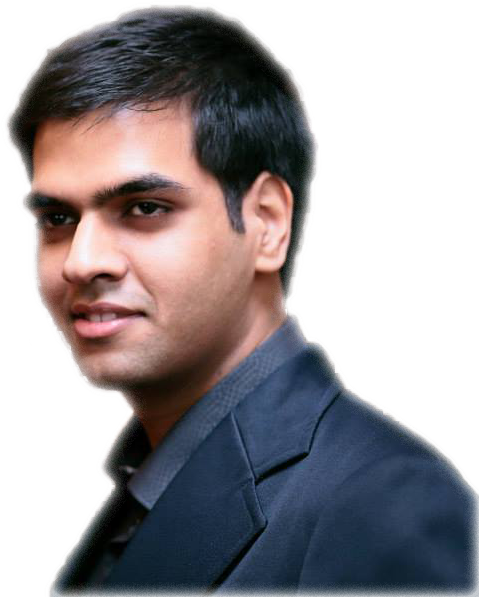
\includegraphics[width=0.8\columnwidth]{kkk}
%	\vspace{-5cm}
%\end{figure}

\begin{flushright} 
	\footnotesize
	\SmallSep
	\CVItemSC{Address}\\%{\bfseries{\color{Plum}{Address}}}\\
	
	105 North-west 103rd St.\\
	Seattle, WA - 98177\\
	\SmallSep
	\CVItemSC{E-Mail}\\%{\bfseries{\color{Plum}{E-Mail}}}\\
	\href{mailto:vicky.p.katara@gmail.com}{\texttt{vicky.p.katara@gmail.com}}\\
	\SmallSep
	\CVItemSC{Mobile}\\%{\bfseries{\color{Plum}{Cellphone}}}\\
	\href{tel:+19842158067}{+1 \(984\) 215 8067}\\
	\SmallSep
		%{\bfseries{\color{Plum}{Website}}}\\
	%\href{http://vickykatara.orgfree.com/}{vickykatara.orgfree.com}\\
	%\SmallSep
	%\CVItemSC{GitHub Repo}\\%{\bfseries{\color{Plum}{Cellphone}}}\\
	%\href{https://github.com/vicky-katara}{\texttt{github.com/vicky-katara}}\\
	\SmallSep
	\CVItemSC{Web}\\%{\bfseries{\color{Plum}{Cellphone}}}\\
	\href{https://vicky-katara.github.io/}{\texttt{vicky-katara.github.io}}\\
	\SmallSep
		\tikz{\draw[loosely dotted,color=Plum,line width=1.5pt](6.2,0) -- (1,0);}
%\end{flushright}\normalsize
%\SmallSep
\CVSection{Technical Skills}
{\footnotesize Java, ML-Ops}\\
{\footnotesize AWS micro-services}\\
{\footnotesize Nvidia riton, AWS-CDK}\\
{\footnotesize Full-Stack Dev}\\
{\footnotesize JavaScript, Web-Dev}\\
\SmallSep
%\end{flushright}\normalsize
\SmallSep
\CVSection{Education}


\CVItem{Masters in \\Computer Science}\\
\begin{footnotesize}
	North Carolina State University
	2015-2016 / G.P.A.: 4.0
\end{footnotesize}
\SmallSep

\CVItem{Bachelors in \\Computer Engineering}\\
\begin{footnotesize}
    University of Mumbai
	2009-2013
\end{footnotesize}
\SmallSep

%\Sep\\
\end{flushright}\normalsize
\tikz{\draw[loosely dotted,color=Plum,line width=1.5pt](6.2,0) -- (1,0);}
\SmallSep
%\begin{figure}
	%\hfill
	%\vspace{-0.3cm}
	\hspace{0.7cm}
		\vspace{-0.35cm}
	\textsc{\bfseries{\color{Plum}{Save My Contact}}}\\\\
	\vspace{+0.45cm}
	%\hspace{-0.4cm}
	
\includegraphics[width=0.8\columnwidth]{qrcode_2.eps}
%\end{figure}
\framebreak

% Right frame
%%%%%%%%%%%%%%%%%%%%
\placetextbox{0.90}{0.995}{\color{Plum}\tiny{Last Updated: Mar 24, 2024}}%

\Huge\bfseries \textsc{\color{Plum} Vicky Katara}
{\normalsize \bfseries  Senior Software Engineer }
\SmallSep

\normalsize\normalfont

% About me
%\begin{Objective}
\begin{footnotesize}
I am a seasoned senior software engineer with experience in building AI/ML Services with AWS Bedrock Gen AI Services using cutting edge technologies solving complex customer problems . I lead teams building products and services in the AWS  AI/ML Org and Amazon Retail product families.
\end{footnotesize}
%\end{Objective}

% Experience
\CVSection{Work Experience}

\CVItem{2021 \textendash \space Present, Senior Software Engineer}\\
\SmallSep
AWS Bedrock Gen AI Services (Computer Vision) \\
{\footnotesize Launched several greenfield Gen-AI Media Processing services. Lead a service migration for AWS Computer-Vision service offerings to reduce Infra-costs by 45\% . Ops-excellence leader for a dev-team with 12 SDEs.\\}

\CVItem{2017 \textendash \space 2021, Software Engineer, Amazon}\\
\SmallSep
Amazon Lists\\
{\footnotesize Project Lead with the Amazon Lists team to deliver several commercially successful products (e.g. Hearts on Amazon Products, Collaborative Lists). Also lead several tech-operational processes within the team.}

% Projects - Start
\CVSection{Projects}
\CVItem{AWS Bedrock GenAI Service Offering }  \RightAlignedInlineText{2024}\\
{\footnotesize Launched a greenfield Gen-AI service offering with AWS Bedrock. This offers customers multi-modal media insight generations using Large-language and classic AI models to offer customers customizable capabilities at desired price-points. \\
	\emph{Technologies Used:} NVidia Triton, Python, Java, AWS-CDK Typescript}%Project-4 End
\SmallSep\\
%Project-new1 Start
\CVItem{AWS Rekognition Labels - Re-architecture} \RightAlignedInlineText{2024}\\
{\footnotesize Delivered a cost-reduction and modernization initiative. This initiative helped reduce Infrastructure costs by 45\%, while also bringing latency improvements of ~15\%. \\color{Black}
\emph{Technologies Used:} NVidia Triton, Python, Java, AWS-CDK Typescript, Python-CV (Pillow, OpenCV}%Project-4 End
\SmallSep\\
%Project-new1 Start
\CVItem{AWS Computer-Vision - Pipeline Health Improvement} \RightAlignedInlineText{2023-2024}\\
{\footnotesize Defined strategy and lead pipeline-health (CI/CD) for the AWS-Computer Vision org. This included ~120 SDEs and ~150 total stakeholders. Eventually reduced deployment effort from 150 developer-days / month to ~26 developer-days per-month}%Project-4 End
\SmallSep\\
%Project-new1 Start
\CVItem{Hearts on Amazon} \RightAlignedInlineText{2024}\\
{\footnotesize Lead the development and launch of Hearts-on-Amazon. This offered an intuitive end-to-end customer experience (including backend-services) that fundamental changes in the amazon retail customer journey.  {Black}
	\emph{Technologies Used:} Java, AWS Elastisearch, JavaScript / Typescript, Java-Spring}%Project-4 End
\SmallSep\\
%Project-new1 Start
\CVItem{Amazon WishLists - Gurupa Migration} \RightAlignedInlineText{2015 - 2022}\\
{\footnotesize Participated and lead the Amazon WishList team's migration off of the Gurupa framework. This included the migration of more than 100 APIs used across many Amazon Retail Web-pages to modern microservices.\\\color{Black}
	\emph{Technologies Used:} Java, Perl-Mason, JavaScript, AWS DynamoDB, etc.}%Project-4 End
\SmallSep\\
%Project-new1 Start
%Project-new1 Start
%Project-5 Start
%\CVItem{Development of Mini-Tennis Game, Mini-Project for Computer Graphics}\\
%{\footnotesize This involved the design and development of 2D Mini-Tennis game.\\ \emph{Technologies Used:} GCC}\\%Project-5 End
%\Sep 
% Projects - End
%%%%%%%%%%%%%%%%%%%%%%%%%%%%%%%%%%%%%
% End document
%%%%%%%%%%%%%%%%%%%%%%%%%%%%%%%%%%%%%
\end{document}